\section{Background}
\label{sec:background}

\begin{comment}
The background's depth and breadth depend on the depth needed to understand your project.
It is not a place to just write about everything you know that is vaguely connected to your project.
The theory is here to help the readers that do not know the theoretical basis of your work, so that they
can gain sufficient understanding to understand your contributions. In particular, the theory section provides
an opportunity to introduce terminology that can later be used without disturbing the text with a definition.

When introducing techniques or results, always reference the source.
Be careful to reference the original contributor of a technique and not just someone who happens to use the technique.%
\footnote{But always make sure that you have read the work you are citing --- if not, cite someone who has!}
For results relevant to your work,
you would want to look particularly at newer results so that you have referenced the most up-to-date work in your area.
If you do not have the source handy when writing, mark in the text that a reference is needed and add it later. \todo{add reference}
Web pages are not reliable sources --- they might be there one day and removed the next; and thus should be avoided, if possible.
A verbal discussion is not a source and should normally not be referenced.
The bulk of citations in the report will appear in Section~\ref{sec:related_work}.
However, you will often need to introduce some terminology and key citations already in this section.
%
You can cite a paper in the following manner (and several other versions,
see the \verb!natbib! package documentation):

\begin{itemize}
    \item when referring to authors:\\
          \citet{Authorson;Bobsen:10} stated something rather nice.
    \item to cite indirectly: \\
          Papers should be written nicely \citep{Authorson;Bobsen:10}
          {\em or\/}\\
          In \cite{Authorson;Bobsen:10}, a less detailed template was presented.
    \item To just cite the authors: \\
          \citeauthor{Authorson;Bobsen:10} wrote a nice paper.
          Or just the year: \citeyear{Authorson;Bobsen:10}.
    \item You can even cite specific pages: \citet[p. 3]{Authorson;Bobsen:10}.
\end{itemize}

You should obviously always cite your teacher's work \citep{BenyonEA:13},
even if it is completely irrelevant \citep{Das;Gamback:13a} or very old \citep{AlshawiEA:91b}.
Digging up an even older book can also appear impressive \citep{Diderichsen:57}.
(Or? ;-)

\subsection{Introducing Figures}

\begin{figure}[t!]
    \centering
    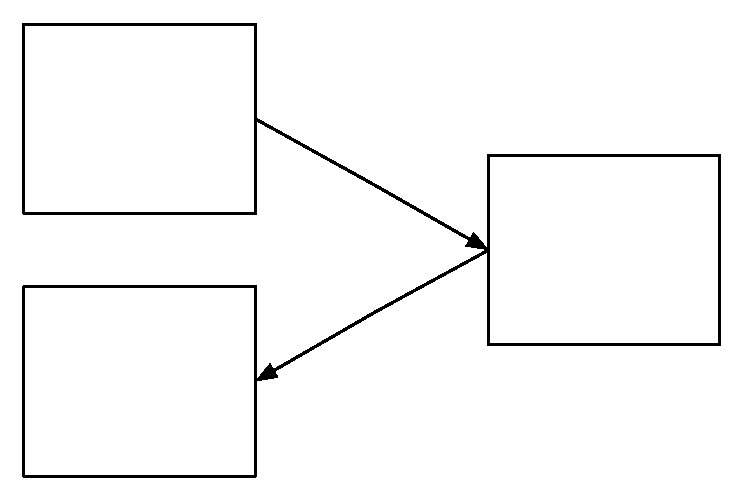
\includegraphics[width=0.5\columnwidth]{figs/figure1.pdf}
    \caption[Boxes and arrows are nice]{Boxes and arrows are nice (adapted from \citealp{Authorson;Bobsen:10}, with permission)}
    \label{fig:BoxesAndArrowsAreNice}
\end{figure}

Remember that when you borrow figures you should always credit the original author --- such as
Figure~\ref{fig:BoxesAndArrowsAreNice} (adapted from \citealp{Authorson;Bobsen:10}),
as well as state that you have permission to reprint it (e.g., if it is published under a Creative Commons License,
or if you have gained explicit permission from the author).

Do not just put the figure in and leave it to the reader to try to understand what the figure is.
The figure should be included to convey a message and you need to help the reader to understand the message
intended by explaining the figure in the text. Hence {\bf all} figures and tables should always be referenced in the text.
There will often be specific parts of a figure or table that you want the reader to pay special attention to (and that you
discuss in more detail in the text). It is helpful if you mark those parts clearly (e.g., by circling them, pointing them out
with arrows, using different colours and fonts, etc.)

It is good practice to add a note about a missing figure in the text,
such as the completely amazing stuff that will appear in Figure~\ref{fig:AmazingFigure}.

Narrow graphics together with the single-column format may lead to large empty spaces.
If you have multiple graphics with related content, it may be preferable to combine them in one graphic.
You can identify the sub-graphics with sub-captions below the sub-graphics numbered (a), (b), (c) etc., and using 9pt text.
The \LaTeX\ packages wrapfig, subfig, subtable and/or subcaption may be useful.

\begin{figure}[t!]
    \centering
    \missingfigure{Here we will add an amazing figure explaining it all}
    \caption{A missing figure}
    \label{fig:AmazingFigure}
\end{figure}

\subsection{Introducing Tables in the Report}

\newcommand\emc{-~~~~}
\begin{table}[t!]
    \centering
    \caption{Example table (F$_1$-scores)}
    \begin{tabular}{c|c|rrrrrr}
        \tabletop
        Langs                  & Source                                           & \multicolumn{1}{c}{Lang1} & \multicolumn{1}{c}{Lang2} & \multicolumn{1}{c}{Univ} & \multicolumn{1}{c}{NE} & \multicolumn{1}{c}{Mixed} & \multicolumn{1}{c}{Undef}
        \\ \tablemid
        \multirow{5}{*}{EN-HI} & FB+TW                                            & 54.22                     & 22.00                     & 19.70                    & 4.00                   & 0.05                      & 0.03                      \\
                               & FB                                               & 75.61                     & 4.17                      & 18.00                    & 2.19                   & 0.02                      & 0.01                      \\
                               & TW                                               & 22.24                     & 48.48                     & 22.42                    & 6.71                   & 0.08                      & 0.07                      \\
                               & Vyas                                             & 54.67                     & 45.27                     & 0.06                     & \emc                   & \emc                      & \emc                      \\
                               & FIRE                                             & 45.57                     & 39.87                     & 14.52                    & \emc                   & 0.04                      & \emc                      \\ \tablemid
        \multirow{2}{*}{EN-BN} & TW                                               & 55.00                     & 23.60                     & 19.04                    & 2.36                   & \emc                      & \emc                      \\
                               & FIRE                                             & 32.47                     & 67.53                     & \emc                     & \emc                   & \emc                      & \emc                      \\ \tablemid
        EN-GU                  & FIRE                                             & 5.01                      & {\bf 94.99}               & \emc                     & \emc                   & \emc                      & \emc                      \\
        \tablemid
        DU-TR                  & Nguyen                                           & 41.50                     & 36.98                     & 21.52                    & \emc                   & \emc                      & \emc                      \\ \tablemid

        EN-ES                  & \multirow{4}{*}{\rotatebox[origin=c]{90}{EMNLP}}
                               & 54.79                                            & 23.50                     & 19.35                     & 2.08                     & 0.04                   & 0.24                                                  \\
        EN-ZH                  &                                                  & 69.50                     & 13.95                     & 5.88                     & 10.60                  & 0.07                      & \emc                      \\
        EN-NE                  &                                                  & 31.14                     & 41.56                     & 24.41                    & 2.73                   & 0.08                      & 0.08                      \\
        AR-AR                  &                                                  & 66.32                     & 13.65                     & 7.29                     & 11.83                  & 0.01                      & 0.90                      \\ \tablebot
    \end{tabular}
    \label{tab:ExampleTable}
\end{table}

As you can see from Table~\ref{tab:ExampleTable}, tables are nice.
However, again, you need to discuss the contents of the table in the text.
You do not need to describe every entry, but draw the reader's attention to what is important in the table,
e.g., that $94.99$ is an amazing F$_1$-score for the English-Gujarati language pair (and that probably something fishy happened there).
\todo[inline]{There is always some more stuff that you will need to add at some later point.
    Be sure to at least make a note about it somewhere.}
\end{comment}

This section will elaborate on technologies central to this project. It is assumed that the reader has basic understanding of what \glspl{acr:lm} are, and also that they are somewhat wandered in the world of \acrfull{acr:nlp}.

\subsection{The Transformer Architecture}

\cite{vaswaniAttentionAllYou2017a} managed to achieve new state-of-the-art results for machine translation tasks with their introduction of the Transformer architecture. The Transformer has later been proved effective for numerous downstream tasks, and for a variety of modalities. Titleing their paper \citetitle{vaswaniAttentionAllYou2017a}, \citeauthor{vaswaniAttentionAllYou2017a} suggest that their attention-based architecture renders \glspl{acr:rnn}  redundant, due to its superior parallellization abilities and the shorter path between combinations of position input and output sequences, making it easier to learn long-range dependencies \citep[6]{vaswaniAttentionAllYou2017a}.

The Transformer employs self-attention, which enables the model to draw connections between arbitrary parts of a given sequence, by-passing the long-range dependency issue commonly found with \glspl{acr:rnn}. An attention function maps a query and a set of key-value pairs to an output, calculating the compatibility between a query corresponding key \citep[3]{vaswaniAttentionAllYou2017a}. Looking at \citeauthor{vaswaniAttentionAllYou2017a}'s proposed attention function \eqref{eq:attention}, we observe that we take the dot product between the query $Q$ and the keys $K$, where $Q$ is the token that we want to compare all the keys to. Keys similar to $Q$ will get a higher score, e.g. be \textit{more attended to}. These differences in attention is further emphasized be applying the softmax function. The final matrix multiplication with the values $V$, being the intitial embeddings of all input tokens, will give us a new embedding in which all tokens have some context from all other words. We improve the attention mechanism by mutiplying each query, key, and value with weigth matrices learned through backpropagation. Self-attention is a special kind of attention in which queries, keys, and values are all the same input sequence.

\begin{equation}
    \text{Attention}(Q, K, V) = \text{softmax}\left(\frac{QK^T}{\sqrt{d_k}}\right)V
    \label{eq:attention}
\end{equation}

Attention blocks can be found in three places \citep[5]{vaswaniAttentionAllYou2017a} in the Transformer architecture (I will use machine translation as example, say, from Norwegian to German):

\begin{enumerate}
    \item In the encoder block to perform self-attention on the input sequence (which is in Norwegian)
    \item In the decoder block to perform self-attention on the output sequence (which is in German)
    \item In the decoder block to perform cross-attention (or encoder-decoder attention) where each position in the decoder attends to all positions in the encoder
\end{enumerate}

The Transformer established a new state of the art in machine translation \cite{vaswaniAttentionAllYou2017a}, and is the fundamental building block of \acrshortpl{acr:lm} like \acrshort{acr:bert}.

\subsection[BERT]{\acrshort{acr:bert}}

\gls{acr:bert} is a family of language models which was first introduced in 2018 and is designed to facilitate a wide range of downstream tasks \citep[5]{devlinBERTPretrainingDeep2019}. The \acrshort{acr:bert} architecture consists of stacked bidirectional Transformer encoders. The self-attention mechanism coupled with a masked language modelling pre-training step allows for training of deep bidirectional representations. 15 percent of words are masked with the special \texttt{[MASK]} token during this pre-training step and left for the model to predict \citep[4]{devlinBERTPretrainingDeep2019}. The second of the two unsupervised tasks used during pre-training, is \gls{acr:nsp}, where the special \texttt{[CLS]} (found at the start of each tokenized sequence) is used to predict if a senctece \texttt{B} follows \texttt{A}. The input representation then looks like this:

$$
    \texttt{[CLS]}\text{ this is sentence A }\texttt{[SEP]}\text{ and this is sentence B }\texttt{[SEP]}
$$

\autoref{fig:bert-high-level-overview} shows a high-level overview of the pre-traning and fine-tuning procedures. For the pre-training, each token of the input sequence, consisting of a sentence pair and the classification token, \texttt{[CLS]}, is transformed into embeddings (vector representations). These per-token embeddings include information of the meaning of the word itself, the meaning of the sentence/segment it belongs to, and the token's position in the full input. These embeddings are the pass through a stack of Transformer encoders (12 and 24 for \textbf{\acrshort{acr:bert}\textsubscript{BASE}} and \textbf{\acrshort{acr:bert}\textsubscript{LARGE}}, respectively), allowing the model to learn more complex patterns and of different granularities (token, sentence, document).

\begin{figure}
    \centering
    \includegraphics*[width=\textwidth]{./figs/BERT_overall_procedures.jpg}
    \caption{High-level overview of the pre-training and fine-tuning procedures for \acrshort{acr:bert} \citep[3]{devlinBERTPretrainingDeep2019}}
    \label{fig:bert-high-level-overview}
\end{figure}

\todo{Fine-tuning}

\subsection[X-Mod]{\acrshort{acr:xmod}}

\gls{acr:xmod} models \citep{pfeifferLiftingCurseMultilinguality2022} attempt to tackle the common problem of multi-linguality in language models. Typically, when one attepmts to train a  language model be multilingual by training on numerous languages, the performance tends to drop after reaching a certain level of performance - \textit{the curse of multilinguality} \citep[1]{pfeifferLiftingCurseMultilinguality2022}.

\subsection{Geodesic Terminology and Metrics}

The evaluation is based upon the Haversine formula, with the Earth's radius is assumed to be 6371 km. The evaluation metric is the median Haversine distance \eqref{eq:haversine} between the predicted coordinates and the ground thruth \citep[4]{scherrerHeLjuVarDial20202020}. A formulation of the Haversine distance can be found on its Wikipedia page\footnote{\url{https://en.wikipedia.org/wiki/Haversine_formula}} where it is described as "the great-circle distance between two points on a sphere given their longitudes and latitudes". The distance $d$ can be expressed as

\begin{equation}
    d = 2r \arcsin\left(\sqrt{\sin^2\left(\frac{\phi_2 - \phi_1}{2}\right) + \cos(\phi_1)\cos(\phi_2)\sin^2\left(\frac{\lambda_2 - \lambda_1}{2}\right)}\right)
    \label{eq:haversine}
\end{equation}

\noindent where $\phi$ and $\lambda$ are latitude and longitude values.

Different map projections were used in the project. The \gls{acr:utm} map projection splits Earth's surface into 60 zones in the latitudal direct and 19 zones in the longitudal direction, forming a grid. Doing this allows us to express coordinates in meters within a grid zone and still obtaining high accuracy measurements. Coordinate values in \acrshort{acr:utm} lie in the six figures, with the easting of the central meridian\footnote{\url{https://gisgeography.com/central-meridian/}} being defined to 500 000 meters to avoid negative easting values within the zone.

The Swiss coordinate system, LV95 \citep{federalofficeoftopographyswisstopoSwissCoordinatesSystem}, was also explored. Its center coordinates are defined to the Swiss capital of Bern and the values lie in the seven figures.
